% This example An LaTeX document showing how to use the l3proj class to
% write your report. Use pdflatex and bibtex to process the file, creating 
% a PDF file as output (there is no need to use dvips when using pdflatex).

% Modified 

\documentclass{l3proj}
\begin{document}
\title{Team R Project Dissertation}
\author{Alex Chilikov \\
        Jacob Ford \\
        Mike Harling \\
        Ivaylo Lafchiev \\
        Mindaugas Ribakauskas \\
        Akos Szente}
\date{1 March 2016}
\maketitle
\educationalconsent
\tableofcontents
%==============================================================================
\chapter{Introduction}
\label{intro}

An introduction, explaining the purpose of the document, a very brief outline of the project and a summary of the structure of the rest of the document (approximately 1-2 pages).

THE REAL INTRODUCTION STARTS HERE

Over the duration of the Team Project 3 course, our team has learned the principles of sound software design, overcome many obstacles, and ultimately completed our project to the best of our ability. This document explores the project to which we were assigned and our journey through the process of gathering requirements, formulating designs, implementing our plans, and deploying the project.

We were assigned to work with the National Health Service in Dumfries Galloway to build a web application which benchmarked different indicators of disadvantages for the area. Our product would be able to, given a locality, sex, age range, and group size, calculate how many of that group one could expect to be disadvantaged in some way, whether they be homeless, have no access to a car or van, lack central heating in their apartment, or any other of the many statistics deemed deprivation criteria. The project involved finding data from several public data sources for Scotland, building a database and importing the gathered data, and creating the front end web application to bridge the gap between our data and the users. The project will be described in greater detail, along with our design decisions and what we achieved, in Chapter \ref{case}.

After the description of the case study, this dissertation will document the key moments of the software development process as a series of reflections. Each reflection will explore one key decision, our reasoning, and what we learned and how we grew as a result of this choice. Finally, we will conclude with more general observations and a section denoting the contributions from each individual member of the team.

THE REAL INTRODUCTION ENDS HERE

The following text illustrates how to cite and input figures.

ALICE \cite{alice} was beginning to get very tired of sitting by her sister
on the bank and of having nothing to do: once or twice she had peeped into
the book her sister was reading, but it had no pictures or conversations in
it, ``and what is the use of a book,'' thought Alice, ``without pictures or
conversations?'

\begin{figure}
\begin{center}

\includegraphics[width=7cm]{figures/alice}
\end{center}
\caption{Behind it was a little door}
\label{fig:alice}
\end{figure}

I've cut the rest of the chapter from Alice. -Jacob

%==============================================================================
\chapter{Case Study}
\label{case}

A description of the case study background and context. This should include a description of the project customer (what was the nature of the organisation you were working for), their objectives for the project, and a summary of what was actually achieved. Where appropriate, this section should also make reference to similar related projects in order to make the context clear (approximately 4-5 pages).

THE REAL CASE STUDY STARTS HERE

\section{Project Description}
\label{description}

One of the key issues the National Health Service has identified in recent years and chosen to address is that of inequalities. Inequalities are measured as conditions which render people disadvantaged; examples include being an unpaid carer and lacking the resources to heat their home. These can have a significant impact on people’s lives and in particular, their health. George Noakes, a statistician for the NHS in Dumfries and Galloway, looked to develop an Inequalities Framework to help organizations across the region ensure that their impact on inequalities is taken into account when delivering services and to make sure services are not exacerbating the problem. These organizations need to be able to benchmark (compare) the populations they are seeing to what might be expected in their area. We were to produce a Benchmarking tool needed so people who engage with the population can measure data they collect versus what should be expected, within a certain statistical range.

George came in to the first interview with a specific idea of what he wanted out of the product. He provided us with a list of deprivation indicators, along with the public data sources where they could be found. In addition, he wanted it to be accessible to anyone who wanted to use it; essentially, everyone in Dumfries and Galloway is a potential user. This includes those running cooking classes for older women, local law enforcement, and data analysts. The product had to be simple enough for anyone to use, but with enough depth so that anyone more interested in the subject could understand the inner workings and do more research of their own. These requirements lent themselves to a web application, an idea on which George was quite keen. His main priorities were simplicity and accessibility so anyone could understand and utilize the data.

\section{Design}
\label{designdocs}

We split the project into three sections: the database, the middleware, and the front end. We decided early on to use mySQL for the database, Spring for the middleware, and Angular for the front end. We began work on these components during first semester, however, it was not until January 2016 that we received the lecture on components and made a component diagram.

\begin{figure}
\begin{center}
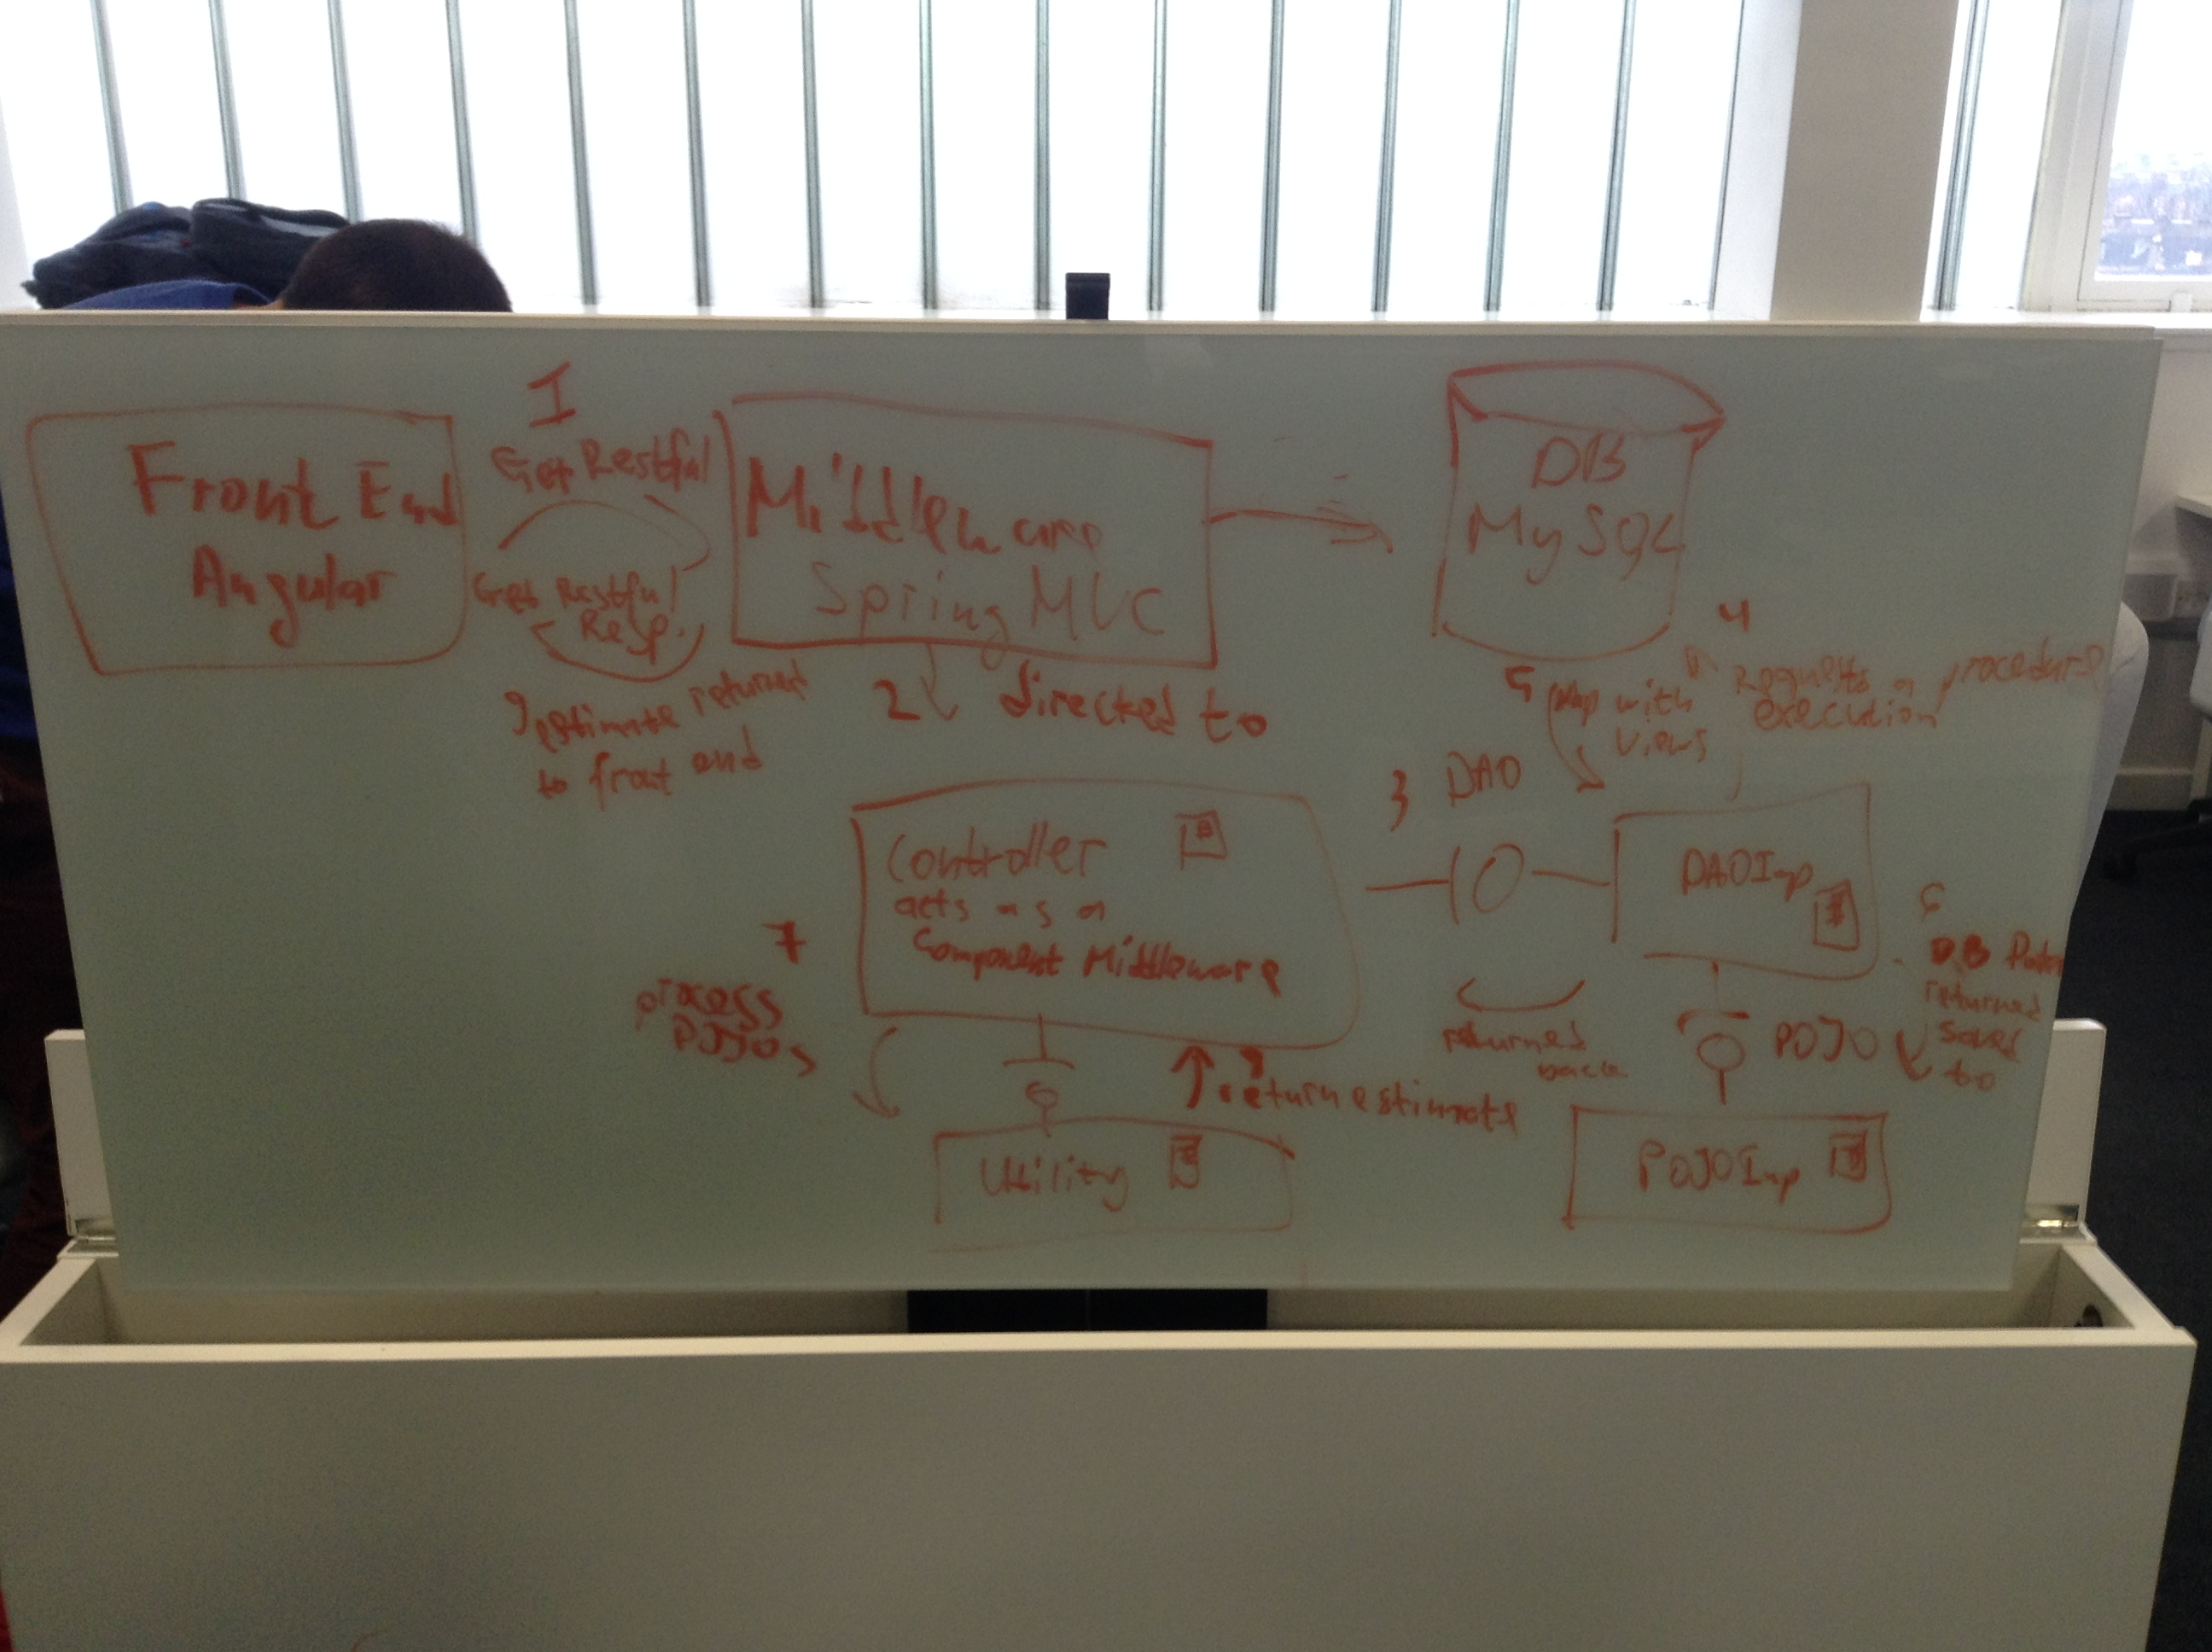
\includegraphics[width=18cm]{figures/component}
\end{center}
\caption{Component Diagram}
\label{fig:component}
\end{figure}

This diagram helped each of us understand how the part we were working on interacted with the rest of the project. It reflected the status of the project at the time and we stuck to this design, maintaining separation of concerns. The components work and interact is as follows:

\begin{itemize}
\item The Client - The client component appears as a separate unit on the left hand side of the picture. It is a representation of a thin client simply requesting HTTP GET Requests and receive a response which is visible using the two-way data binding of AngularJS.

\item The Web Services Server - the Spring MVC Web Services Server appearing in the middle is using a middleware in our communication between the Client and DB server. The Spring Server itself is constructed of different components presented below it.

\item The Controller - it has controllers responsible for managing individual requests to specific URL as we have a 1:1 mapping between a HTTP GET Request and controller handling the request. Inside the Spring system we can imagine the controller as the middleware.

\item The DAO - it channels the request to a DAO (Data Access Object) which sends the request to the correct DB Server and procedure for processing and collects the result storing it in an internal structure using the POJO.

\item The POJO - POJO is an abstraction, a component addressing the representation of the tuples from the view received from the DB.

\item The Utility - Once the controller gets the DS of POJOs it passes the processing of this data to the suitable utility class for analyzing. The utility class conducts the processing of the data using the correct equation for probability analysis. After the results is produced, the controller sends back the response for visualization in the browser. 
\end{itemize}

\section{What We Achieved}
\label{achievements}

What did we achieve? Who knows. I will fill in this section after our final demonstration. -Jacob

%==============================================================================
\chapter{Reflections}

Several sections that reflect on your experiences during the team project. Each section should discuss one theme, characterised by incidents or events that occurred during the team course of the project from which you learned (approximately 12-15 pages).

Reflecting on your practice is the hardest part of writing the dissertation, so you are encouraged to talk to the course coordinators and demonstrators to find out what you could include in this section. A good source of examples of incidents for reflection is often the documentation from your retrospectives, because you used the retrospectives to identify areas of your process that could be changed or done better. You should also, try to relate your experiences to other studies available in the software engineering literature (the recommended reading is a good starting point for this).

For example, if you found that you had to drop a feature during an iteration, discuss the reasons why the feature had to be dropped. Had you given yourselves too much work? Was the feature harder to implement than you realised? Had you got your priorities wrong? Then consider looking at the literature (see the recommended reading for PSD3) on project planning and estimation. Was your experience typical of a software project? What steps do other developers advocate for improving estimation?

Alternatively, did you have to make some big design decisions or choice of software platforms early on in the project? What impact did these choices have? Were they the right ones? How might you have improved the decision making process to reduce uncertainty? Did you implement a prototype before proceeding to far with the main implementation? How much effort did this involve? What did you learn about the platform as a result?

\section{The Premature Design Decision}
\label{design}

(alex-note - introduction of the reflection - what it is about and summarizing what we will talk about
-the issue
-practices used
-what we learned
-our experience during the process
)
The first reflection we would like to discuss as part of the reflection chapter is about the premature design decisions which were made as part of our software engineering process, the practices we used, and what we learned and changed about them as a result of the difficulties we experienced during the process.

(Introduce the reflection better explain the situation )
The premature design decision refers to the fact that both the front and back ends of the application were develop to expect separate execution paths for different deprivation criteria.(introduction of reflection) The reason for implementing both parts in this way was as initially it was considered that each deprivation criterion can have different data related to it and different search parameters, potentially distinctive analyser (justification of mistake). This justification can lead us to several possible paths for a  discussion.

(justification why  it was expected different deprivation criteria to have different data
-assumptions
-probable misunderstanding
-lack of thorough documentation
-bad initial requirements gathering
-meeting only 30 minutes
)
Firstly, the different data related to different criteria was an assumption made by the team at the begining of the application processes. Most likely, as it was later discussed with the teammates, this was due to the fact that this requirement was not initially discussed with the client, an often observed situnation in which software developers make premature design desicions caused as a result of misunderstanding or introducing of an assumption either from the client or the software development team later significantly affecting the project (QUOTE)(premature assumptions and misunderstanding duing an initial meeting). Another potential reason is the lack of thorough documentation at the beginning of the software process. The lack of such documentation lead to the hiding of the assumption which could have been potentially avoided if an appropriate thorough documentation was present to reveal it(initial lack of documentation - maybe QUOTE). A third potential explanation for the trouble can be explored as part of the initial requirements gathering activity(bad initial requirements gathering - quoute). A more complete requirements elicitation with regard to the type of data expected could have potentially prevented the issue. If we had investigated what data exactly we could expect for each of the deprivation criteria during the meeting, such a misunderstanding could have been avoided. Furthermore, the lack of time, due to the limitation of the 30 minute initial meeting is an additional explanation we can analyse as a cause. A possible way for preventing it is an improvement of the communication between the team and the client using more frequent exchanges of emails.

(expect different search criteria for different criteria)
Secondly, the presence of different search parameters for different deprivation criteria was another argument to use different work flows for each deprivation criterion. This later turned out to be a wrong assumption, as some of the potential reasons for this can be identified in the following alternatives. Perhaps the most significant of the them is the lack of understanding of the project and more precisely what can be expected from a benchmarking tool from the point of view of the client. One way for avoid this in future project is potentially presenting prototypes(quote- why this is good) or expecting from the client to show us other projects as closely related to what he expects as possible(quote). Alternatively, a further reading about the project objectives would have additionally contributed for avoiding such mistakes in future (quote).

(different analyser)
The final potential reason for the expected separate work flows for each deprivation criterion can be found in the expectation of different analysers. The analysers are the classes responsible for the business logic of the back end, they provide the estimates for a particular deprivation criterion selection. It was not initially known what type(ies) of statistical distribution(s) will be used, whether the users will be able to choose them and correspondingly if they will be allowed to modify the confidence interval.  All of these assumptions were not well considered and were not realized as assumptions instead it was simply considered that this should be the expected way the application to be done providing this functionality, which later was discovered not to be the case. A potetial edifying conclusion of these facts can be that prior planning is important and that the project development team should have first better identify the requirements, clarify and discuss them for confirmation with the customer instead of making premature assumption. It would have been better if the time spend coding at the begining of the design process was spent better understanding and planning the scope of the application.

(impact)
In this paragraph the impact of the premature design decision will be discussed. Once the reasons for its manifesting are identified, the complete impact of the decision will help the reader better understand why the particular choices were taken to deal with the situation. First, one of the major impacts was the cost related to implementing the separate work paths for each of the deprivation criteria. The separate work paths led to repetition of code both in the front and back end when this time could have been better spent for resolving other tasks. Additionally to this, the increased number of classes in the back end needed more thorough testing (a test for each class) which similarly was a repetition of code and waste of time for the team. Finally, the use of separate execution paths for different deprivation criteria led to increased complexity and consequtively more expensive maintenance.

Fortunately, the premature design decision leading to the negative impact described above had positive effects as well. It introduced a trade-off between complexity and time related cost and flexibility, opportunities for improvement and easier maintanence. In this paragraph the advantages of using separate paths are presented. Firstly, as stated above the overall flexibility of project was improved as a result of the premature design decision. It made possible different Analyser classes to me introduced for different deprivation criteria to allow their estimation to be handled separately in case we have different data for different deprivation criteria. Even if it is not the case now, it can potentially be in the future. This is particularly important fact as the application is a heavily related to its data - it is a benchmarking tool, so flexibility related to different analysers is extremely useful feature. More specifically, each of the analysers can use a different statistical distibution equation based on the different type of deprivation criteria for providing more accurate results for providing reliable estimates which can be the only case for some deprivation criteria and data distributions. As an example, if a new deprivation criterion is introducted with limited data the current uniform distribution schema is not a suitable probabilistic solution. In such a scenario other distribution equations must be adopted. As discussed with the client, there is a long list of additional parameters required from him which will not be implemented as part of the current release due to the lack of time. Secondly, the use of different execution paths provides alternative search mechanisms and parameters. More specifically, using subparamaters for different deprivation criteria is a possible extra search mechanism refining the search and providing more flexibility as part of an advance search for example. The idea of subparameters appear as part of the final product but is left a "read-only" functionality which is not functioning at the moment because of the lack of more precise data and sources such a a more precise data can be imported from.

(What changed in the project team (if anything) as a result of the experience?)
aus
As a final part of this reflection, we would like to present the changes we did as part of our software engineering processing as a result of the experience. First, we significantly improved our interviewing processes meeting in advance and discussing what we will talk during the meetings presenting our progress, which was allowing any assumption to be identified in time and prevented before they become a considerable part of the application. Additionally, we adopted a practice to document all of our meetings with the client and disucss our understing of the new features to be implemented during the next iteration cycle. As a proof of this you can look at the team R moodle page. The complete documentation of meetings made it  possible to better understand what it is expected from us. As a particularly appropriate example we can look at the second interview documentation wiki. There two sections there which are particularly relevant, namely ALGORITHM FOR OUTPUT and COMMENTARY ON PROTOTYPE. The algorithm for output section explains in detail the way the analyser classes from above must be designed and resolve potential issues with assumptions related to using more than one analyser, different confidence intervals, and distribution equations making it clear how the estimation must function to prevent introduction of further assumption. The second section the COMMENTARY ON PROTOTYPE refers to the prototype we created to similarly decrease the number of assumptions, premature design decision and the cost associated with them. The prototype was particularly useful way prevent premature design decisions with respect to the front end in particular. Additionall, documenting the feedback given from the client for the prototype made it straightforward to confirm his expectations about the front end and later design and implement it feelng confident that our implementation is what is expected and desired by the customer.

To conclude this reflection, the premature design decision lead to additional work and following financial cost related to this. They were mainly caused by poor documentation, assumptions, and bad interview practices. All of this potential causes were limited using prototypes for removing assumptions and getting approval by the client, improved documentation and better interview methadologies. Overally, the premature design decisions provided a great amount of flexibility as well such as opportunity for adding alternative distribution equations, different confidence intervals, and deprivation criteria subparameters. In brief, the premature design decisons caused some potential difficulties but they helped us learn a lot and improve our software engineering process as supported by the arguments above.
 
 


The following diagrams (especially figure \ref{fig:alice}) illustrate the
process...

\section{Repeated Code in the Front End}
\label{repeated}

One cause of significant debate was regarding the code of the front end as we were passing through to refactor and optimize. When we first wrote the code, each of the deprivation criteria required different parameters, due to how some data was divided into gender and age groups, as described in small detail above. However, we later learned that our assumption was incorrect and that the client preferred us to use estimation to compensate for the lack of gender and age division in some of the data, which meant that each deprivation criterion took in the same parameters from another part of the page. We saw this when refactoring, as each of the criteria had their own controller, and a debate ensued. Some argued that by traditional refactoring practices, we should turn all of those methods with the same parameters which all returned data in the same format into one method which takes an additional parameter, which indicates which database procedure to use, which was then the only difference in the way the different criteria functions operated. However, others argued that should we decide to increase functionality for some of the criteria later, we would vastly benefit from keeping the methods separate. For example, if we decided to let users break down ethnicity as a criteria into its three components: South Asian, Black Afro-Carribean, and White Gypsy or Traveler, being able to add this functionality directly to the method for getting the ethnicity results would be much easier than if we amalgamate all of the different methods into one. Eventually, the latter argument favoring a format better for maintenance and future development won, and the similar methods remained separate.

We learned from this the value of bringing a critical eye to the refactoring process rather than blindly refactoring every bit of code possible. It is important to think ahead when developing in order to ensure that the code you produce can be maintained and improved if need be, should requirements change.

This led to an overall change in the way in which the team approached problems and developments, as it made us more aware that we need to keep code as flexible as possible and ensure that it is both maintainable and open for further development.

%==============================================================================
\section{Implementation}
\label{impl}

These next few sections are from the example tex file.

In this chapter, we describe how the implemented the system.

%------------------------------------------------------------------------------
\section{User Interface}

Blah blah blah
Blah blah blah
Blah blah blah
Blah blah blah

% - - - - - - - - - - - - - - - - - - - - - - - - - - - - - - - - - - - - - - -
\subsection{Foo}

Blah blah blah
Blah blah blah
Blah blah blah
Blah blah blah

%------------------------------------------------------------------------------
\section{Database Model}

\begin{enumerate}
\item Blah blah blah
\item Blah blah blah
\item Blah blah blah
\item Blah blah blah
\end{enumerate}



%==============================================================================
\section{Evaluation}

We evaluated the project by...

%==============================================================================
\chapter{Conclusion}

A conclusion that draws general and wider lessons from the case study (approximately 1-2 pages).

%==============================================================================
\section{Contributions}

Here we explain that Lewis Carroll wrote chapter \ref{intro}. John Wayne
was out riding his horse every day and didn't do anything. Marilyn Monroe
was great at getting the requirements specification and coordinating the
writing of the report. Betty Davis did the coding of the kernel of the
project, described in Chapter \ref{impl}.  James Dean handled the
multimedia content of the project.

%==============================================================================
\bibliographystyle{plain}
\bibliography{example}
\end{document}
